\documentclass{article}

% New commands declaration

\usepackage[french]{}
\usepackage[T1]{fontenc}

\usepackage{natbib,bibentry}
\usepackage{color}
\usepackage{yfonts}
\usepackage{graphicx}
\usepackage{epsfig,subfigure}
\usepackage{amsmath,amssymb,amsfonts}
\usepackage{calc}
\usepackage{float}

\usepackage{array}
\newcolumntype{L}[1]{>{\raggedright\let\newline\\\arraybackslash\hspace{0pt}}m{#1}}
\newcolumntype{C}[1]{>{\centering\let\newline\\\arraybackslash\hspace{0pt}}m{#1}}
\newcolumntype{R}[1]{>{\raggedleft\let\newline\\\arraybackslash\hspace{0pt}}m{#1}}


\DeclareGraphicsExtensions{.eps, .jpg, .png}

\parindent = 0mm

\bibliographystyle{plain}

\hoffset = -20mm
\voffset = -25mm
\textwidth = 160mm
\textheight = 240mm

% \definecolor{lightgray}{gray}{0.2}


\newcommand{\expect}{{\rm I \mkern-2.5mu \nonscript\mkern-.5mu E}}
\newcommand{\equaldef}{\stackrel{d}{=}}
\newcommand{\argmax}{\operatornamewithlimits{argmax}}

\newcommand{\dnu}{16}
\newcommand{\solskip}{10mm}

\renewcommand{\topfraction}{1}
\renewcommand{\bottomfraction}{1}
\renewcommand{\textfraction}{0}

\newcommand{\debutrep}[1]{\color{blue}\begin{center} \hrulefill \textbf{ #1 } \hrulefill \end{center} }
\newcommand{\finrep}{\vspace*{5mm}\hfill $\square$\color{black}\vspace*{5mm}}


\begin{document}

\baselineskip = 4mm
\title{Traitement des Signaux Aléatoires \\
Estimation Spectrale}
\author{\textbf{4 ETI -- CPE Lyon }\\[3mm]
{Travaux Pratiques TSA}}
\date{}

\maketitle

\noindent\fbox{
\parbox{\linewidth-2\fboxrule-2\fboxsep}
{ 
\vspace*{2mm}
{\large\bf Noms, Prénoms: BURNOT Jean-Christophe, LANGUILLE Antoine}\\[3mm]
{\large\bf Groupe: D}\\[3mm]
{\large\bf Date: 29 Novembre 2022}\\[2mm]}}
\vspace*{5mm}


\textbf{\Large Objectifs du TP}\\[4mm]

\begin{list}{-}{\setlength{\leftmargin}{3mm} \setlength{\labelwidth}{20mm} \setlength{\labelsep}{2mm} \setlength{\itemsep}{1mm} }
\item Comprendre la notion de densité spectrale d'énergie ou de puissance moyenne
\item Manipuler différents estimateurs empiriques (à partir d'une série temporelle de taille finie) de DSE/DSPM
\item Etudier l'effet du compromis biais-variance d'un estimateur
\end{list}

\textbf{\Large Notes post scriptum}\\[4mm]
Une erreur s'est glissée dans les graphiques des simulations, les légendes "théoriques" et "biaisées" ont été inversées.

Les tracés théoriques sont alors en couleur en orange / rouge et les tracés biaisés, prenant en compte la limitation temporelle apparaissent en jaune.\newline

La simulation théorique repose sur une analyse d'une infinité de réalisations de signaux aléatoires d'une longueur infinie, son atténuation en bande atténuée tends vers l'infini (tracés rouge).En revanche, la limitation temporelle entraine la périodisation en fréquence du signal, cette atténuation idéale est alors inatteignable et l'atténuation stagne alors autour d'une valeur en bande atténuée (tracés jaune).

\vspace*{5mm}

\section{Préparation}

\begin{itemize}
\item[{\bf Question 1}] Comment peut-on calculer simplement la densité spectrale d’énergie (DSE) d’un signal certain d’énergie finie ?

\debutrep{réponse}
Pour un signal d'énergie finie, la Densité Spectrale d'Énergie est égale à 
\[\Gamma_x(\nu) = E(\nu)^*E(\nu)\]

\finrep

\item[{\bf Question 2}] Comment est définie la densité spectrale de puissance moyenne (DSPM) d’un processus aléatoire ?

\debutrep{réponse}
La DSPM d'un processus aléatoire est défini grâce au théorème de Wiener-Kitchine
\[
\Gamma_s(\nu) = TF(\gamma_s(\tau))
\]
\finrep

\item[{\bf Question 3}] Quelles sont les grandeurs qui permettent de chiffrer la qualité d’une estimation dans le cas général ? et la qualité de l’estimation spectrale en particulier.

\debutrep{réponse}
On chiffre la qualité d'une estimation grâce à 4 grandeurs
\begin{itemize}
    \item Le biais d'estimation
    \item La variance de l'estimateur
    \item La précision d'estimation
    \item La résolution fréquentielle
\end{itemize}
\finrep

\item[{\bf Question 4}] Exprimer la densité spectrale de puissance moyenne (DSPM) GB ( f ) d’un bruit blanc stationnaire centré.

\debutrep{réponse}
Un bruit blanc est à corrélation microscopique, sa fonction d'autocorrélation $\gamma_B(\tau)$ se résume donc à un Dirac, ce qui dans le domaine fréquentiel se traduit par une constante. \\
De plus on a $\gamma_s(\tau) = \bar{P_X}$. \\
Ainsi
\[
\Gamma_B(f) = \Gamma_0 = \bar{P_X}
\]

\finrep

\item[{\bf Question 5}] Exprimer GX ( f ) , où X(t) est la sortie d’un filtre excité par un bruit blanc centré, en fonction de la DSPM du bruit blanc et des caractéristiques du filtre.

\debutrep{réponse}
\[
    \begin{split}\\
        \Gamma_X(f) &= TF(\gamma_X(\tau))       \\
        &= TF\left((\gamma_B * h)(\tau)\right)  \\
        &= TF\left((\Gamma_0.\delta * h)(\tau)\right) \\
        &= \Gamma_0.1.H(f)
    \end{split}
\]
\finrep

\item[{\bf Question 6}] En une phrase (sans formule), décrire le procédé de calcul de la DSPM estimée G1 ( f )
d’une séquence aléatoire via l’estimateur simple.

\debutrep{réponse}
Avec un estimateur simple, la transformée de Fourier de nos échantillons, puis on l'éleve au carré avant de la diviser par le nombre de points.
Ce calcul revient à diviser la Densité Spectrale d'Énergie par le nombre d'échantillons.
\finrep

\item[{\bf Question 7}] Rappeler le mode de graduation d’une TFD-N points en fréquences réduites.
\debutrep{réponse}
Une TFD-N points est graduée de $0$ à $1 - \frac{1}{N}$ pour un pas égal à $1\over N$
\finrep

\item[{\bf Question 8}] Décrire (avec une phrase) le procédé de calcul de la DSPM estimée G2 ( f ) d’une
séquence aléatoire via l’estimateur moyenné.

\debutrep{réponse}
On découpe le signal en plusieurs tranches, on calcule la Densité Spectrale d'Énergie de chaque échantillon que l'on divise par le nombre d'échantillons dans chaque tranche.\newline
On obtiens alors autant d'estimations de DSPM que de tranches. On moyenne ensuite ces estimations pour obtenir notre estimation finale.
\finrep

\item[{\bf Question 9}] Que signifie le terme «compromis biais-variance» dans le cas de l’estimateur moyenné ?

\debutrep{réponse}
Le compromis biais-variance dans le cas de l'estimateur moyenné caractérise l'évolution inversement proportionelle du biais et de la variance de l'estimateur en fonction des paramètres (ici la largeur M).
\finrep

\item[{\bf Question 10}] Quelles modifications sont apportées au procédé de calcul de l’estimateur de Welch par rapport à l’estimateur moyenné ?

\debutrep{réponse}

L'estimateur de Welch autorise le recouvrement des bandes de découpages de l'estimateur moyenné. On applique également une fenêtre différente de la porte à ces tranches avant d'en calculer la DSE, pour réduire au maximum les parasites dûs à la convolution fréquentielle engendrée par la limitation temporelle.

\finrep

\end{itemize}

\clearpage
\setcounter{section}{2}
\section{Estimation de la DSPM d'un bruit blanc gaussien filtré}
\subsection{Génération du bruit à analyser}

A quoi sert l'entier permettant d'initialiser le générateur ?

\debutrep{réponse ci-dessous}
La génération de nombre pseudo-aléatoires se fait à partir d'une "graine" (seed) qui est par défaut la valeur de l'horloge système à l'exécution. Cette valeur permet le caractère suffisament aléatoire de la génération de nombres entre deux exécutions.

Fixer ce nombre empêche la variation inter-exécutions, garantissant ainsi un signal aléatoire lors de l'exécution mais identique entre les différentes exécutions.

On peut alors comparer les performances de plusieurs estimateurs, sachant qu'ils estimeront le même signal.
\finrep

\subsection{Estimateur spectral simple}
\subsubsection{Script de la fonction {\tt Matlab} développée}

\debutrep{code ci-dessous}
\begin{verbatim}
function [Gamma, f, N] = simpleDSPM(X, nd, nf, NFFT)

ana = X(nd:nf);
N = nf - nd; %Indices de début et de fin de sélection

% On fait la transformé de fourrier N-points
Xf = fft(ana, NFFT);
f = [0 : 1/NFFT : 1-1/NFFT];

% On calcule la DSPM (DSE divisée par nombre d'échantillons)
Gamma = (1/N).*abs(Xf).^2;
end
\end{verbatim}
\finrep

\subsubsection{Expérimentation}

\begin{enumerate}
\renewcommand{\theenumi}{\Alph{enumi}}
\item Etude du biais et de la variance en fonction du nombre $N$ d'échantillons de bruit

\debutrep{figures ci-dessous}

\begin{figure}[H]
\centering
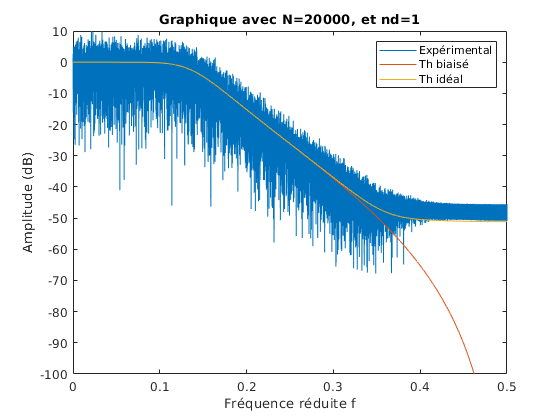
\includegraphics[width=0.75\columnwidth]{Variation-longueur-simple.png}
\caption{$N$ faible -- indice de début de la séquence à 1}
\end{figure}

\begin{figure}[H]
\centering
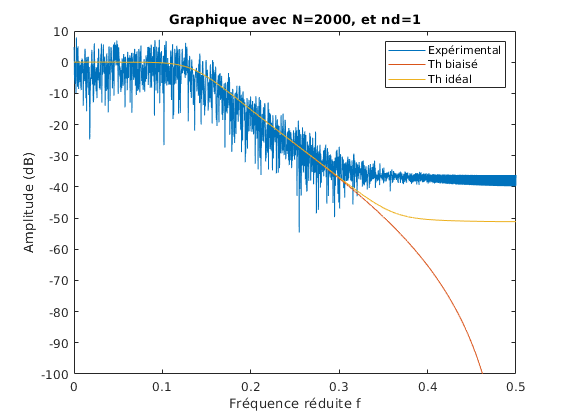
\includegraphics[width=0.75\columnwidth]{Variation-longueur-simple-2.png}
\caption{$N$ élevé -- indice de début de la séquence à 1}
\end{figure}
\finrep

Commentaires.

\debutrep{réponse ci-dessous}
Lorsque N augmente, on observe une diminution de la variance du signal (trace plus "épaisse") mais également une augmentation du biais ous la forme d'écart entre la valeur biaisée et la valeur expérimentale.
\finrep

\item Etude du biais et de la variance en fonction de la réalisation considérée, à $N$ fixé

\debutrep{figures ci-dessous}

\begin{figure}[H]
\centering
\includegraphics[width=0.75\columnwidth]{Variation-depart-simple.png}
\caption{$N \sim 1000$ -- indice de début de la séquence à 1}
\end{figure}

\begin{figure}[H]
\centering
\includegraphics[width=0.75\columnwidth]{Variation-depart-simple-2.png}
\caption{$N \sim 1000$  -- indice de début de la séquence fixé à une autre position ($\gg 1000$) dans la séquence}
\end{figure}
\finrep

Commentaires.

\debutrep{réponse ci-dessous}
Dans notre deuxième figure, notre réalisation expérimentale est bien plus proche de l'idéal.\\
On tire comme conclusion que pour avoir une estimation correcte (moins de biais), il est préférable de ne pas démarrer notre séquence à 1.

Cette varation montre la variation statistique entre les différentes parties du signal, soulignant ainsi que le signal ne respecte pas la propriété de stationnarité.

On préférera alors se limiter à un nombre fixé d'échantillons commencant à un indice fixe pour comparer les estimations.
\finrep

\item Etude du biais et de la variance en fonction du nombre $NFFT$ de FFT

\debutrep{figures ci-dessous}

\begin{figure}[H]
\centering
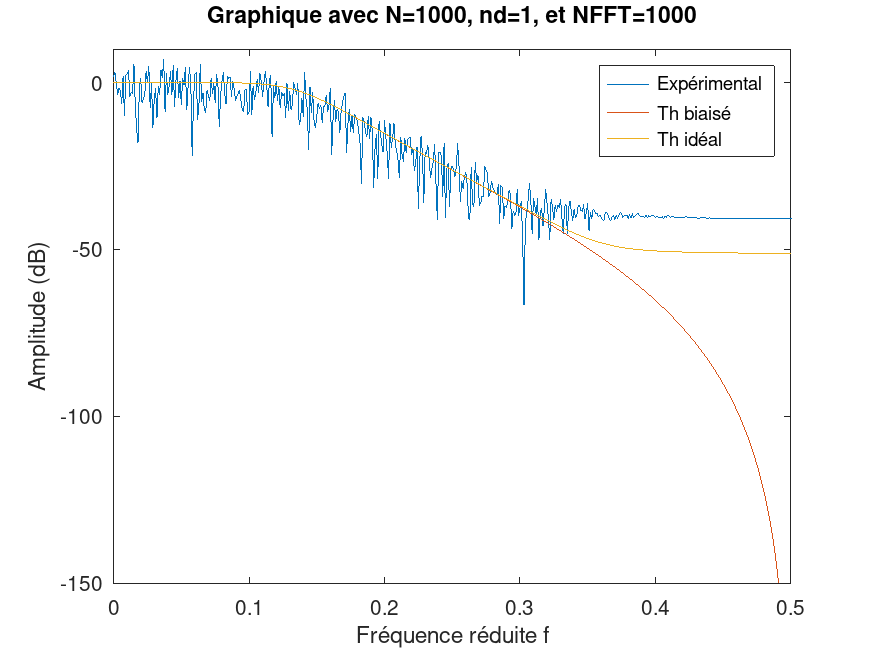
\includegraphics[width=0.75\columnwidth]{Variation-NFFT-simple.png}
\caption{$N$ constant -- indice de début de la séquence à 1 -- $NFFT \sim N$}
\end{figure}

\begin{figure}[H]
\centering
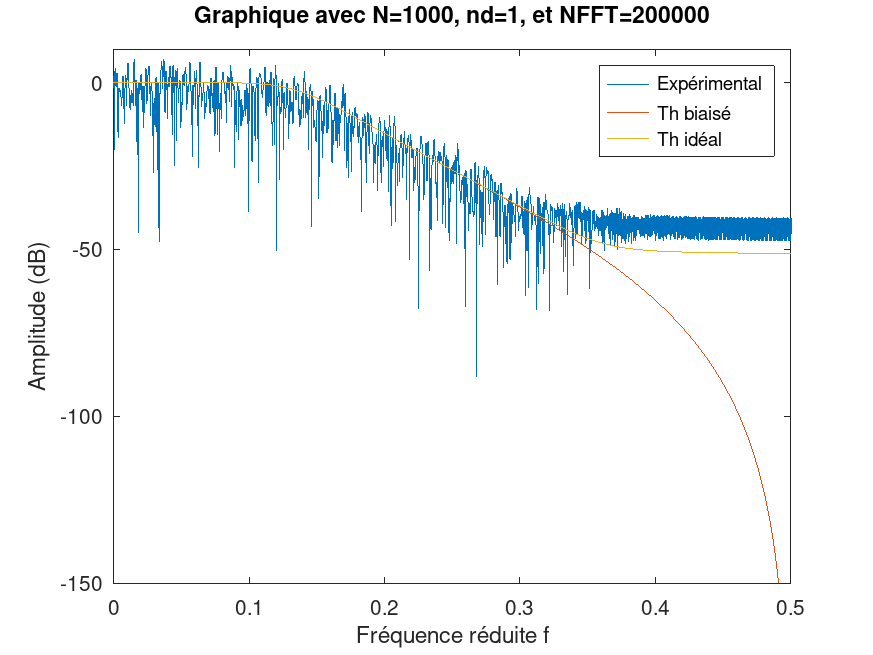
\includegraphics[width=0.75\columnwidth]{Variation-NFFT-simple-2.png}
\caption{$N$ constant -- indice de début de la séquence à 1 -- $NFFT \gg N$}
\end{figure}

\finrep

Commentaires.

\debutrep{réponse ci-dessous}
On observe une augmentation de la variance du signal lorsque le nombre de points de la FFT devient grand.
Il semble qu'avoir N et NFFT au même ordre de grandeur nous fournisse la meilleur lisibilité.
On ne peut aller en dessous du nombre d'échantillons N, au risque de perdre de l'information sur la FFT.
\finrep

\item Conclusion
Quel est le principal défaut de l'estimateur simple ?

\debutrep{réponse ci-dessous}
L'estimateur simple a pour principal problème son biais élevé. Surtout pour les hautes fréquences. Peu importe la grandeur sur laquelle on influe, on constate un biais élevé pour les hautes fréquences de par le caractère fini (Courbe rouge et courbe jaune écartées).
\finrep

\end{enumerate}

\clearpage
\subsection{Estimateur spectral moyenné}

\textbf{On fixera $\mathbf{N=4096}$ dans tout ce qui suit.}

\subsubsection{Script de la fonction {\tt Matlab} développé}

\debutrep{code ci-dessous}
\begin{verbatim}
function [Gamma, f] = moyenneurDSPM(X, N, M, NFFT)
    ana = X(1:N);
    window = rectwin(M);
    [Gamma, f] = pwelch(ana,window,0,NFFT, 1, "twosided");
end
\end{verbatim}
\finrep


\subsubsection{Expérimentation}

En précisant bien la valeur des paramètres utilisés pour les essais, affichez les figures correspondantes aux conditions indiquées.
\debutrep{figure ci-dessous}

\begin{figure}[H]
\centering
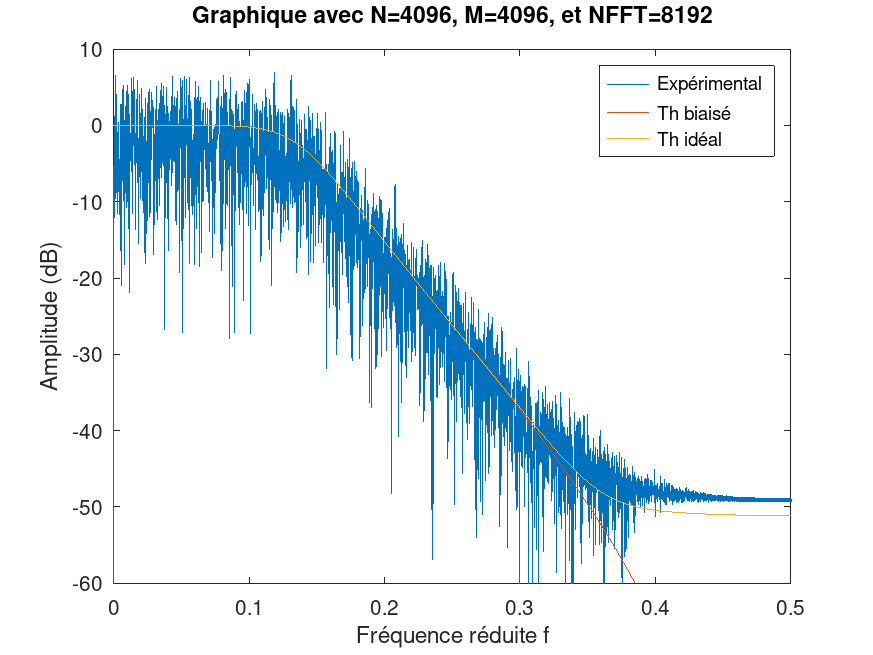
\includegraphics[width=0.75\columnwidth]{Variation-M-moyenneur.png}
\caption{$N=4096$ -- tranches courtes $M = 4096$, $NFFT = 8192$}
\end{figure}
\finrep

Commentaires
\debutrep{réponse ci-dessous}
L'utilisation de tranches courtes ($M$ petit) c'ést à dire d'un nombre de segments $L$ élevés. A pour effet d'augmenter la résolution fréquentielle. Le biais est diminué par rapport à l'estimateur simple mais la variance est plus élevée.
\finrep

\debutrep{figure ci-dessous}
\begin{figure}[H]
\centering
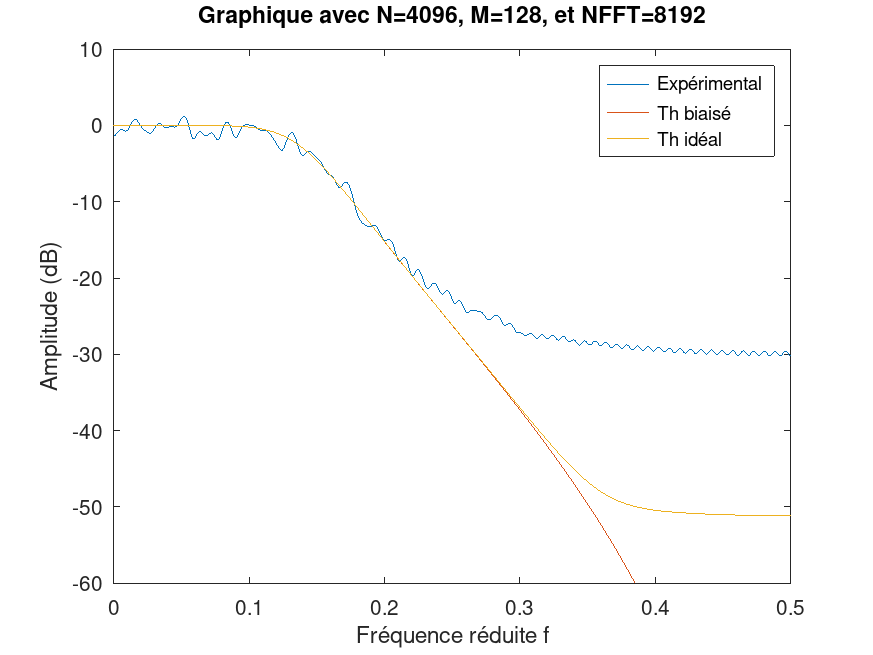
\includegraphics[width=0.75\columnwidth]{Variation-M-moyenneur-2.png}
\caption{$N=4096$ -- tranches longues $M = 64$, $NFFT = 128$}
\end{figure}

\finrep

Commentaires
\debutrep{réponse ci-dessous}
L'utilisation de tranches longues ($M$ grand) c'ést à dire d'un nombre de segments $L$ faible. A pour effet de diminuer la résolution fréquentielle. La variance est moins importante mais le biais augmente significativement.
\finrep

\debutrep{figure ci-dessous}
\begin{figure}[H]
\centering
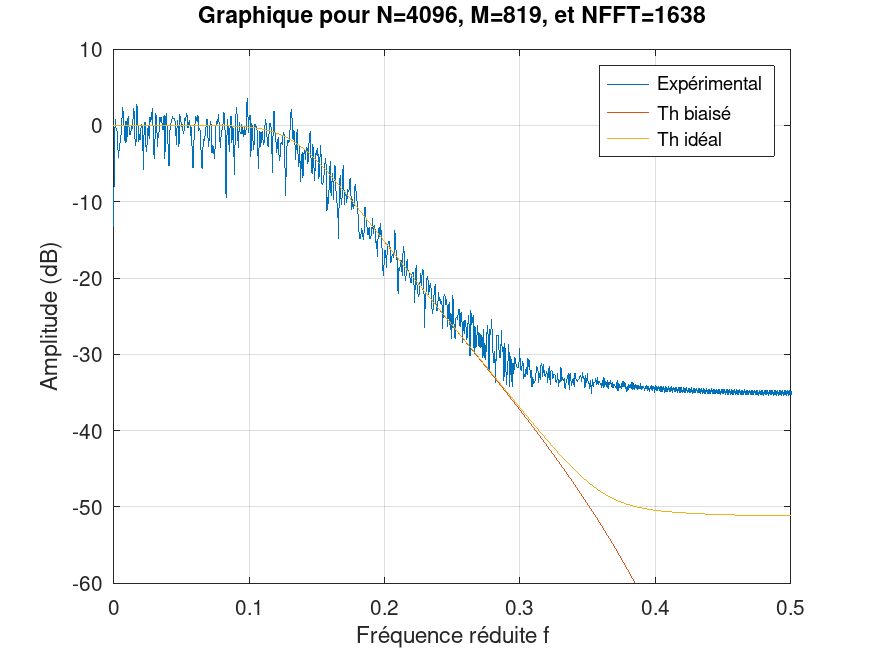
\includegraphics[width=0.75\columnwidth]{Variation-M-best.png}
\caption{$N=4096$ -- Meilleur compromis biais variance atteint pour $M = 819$, $NFFT = 1638$}
\end{figure}

\finrep

Quelle information permettrait d'obtenir le meilleur compromis biais-variance? 

\debutrep{réponse ci-dessous}
Le meilleurs compromis biais-variance peut être atteint en connaissant la valeur de l'écart-type du signal selon la formule:
\[
L = \Delta_{x_{opt}} \approx 3.49 \hat{\sigma_x} N ^ {-1\over3}
\]
\finrep
\clearpage
\section{Estimateur de Welch}

\subsection{Etude préalable des fenêtres}

Quelles différences de comportement fréquentiel peut-on observer pour les 6 fenêtres proposées (lobe principal, lobes latéraux\ldots).

\subsubsection{Script de la fonction {\tt Matlab} développée}

\debutrep{code ci-dessous}
\begin{verbatim}
function [Gamma, f] = welchDSPM(X, N, Nom_fenetre, M, NOVERLAP, NFFT)
  ana = X(1:N);
  WIN = eval([Nom_fenetre, "(M);"]);
  [Gamma, f] = pwelch(ana, WIN, NOVERLAP, NFFT, 1, "twosided");
end
\end{verbatim}
\finrep

\subsubsection{Expérimentation}

\begin{enumerate}
\renewcommand{\theenumi}{\Alph{enumi}}

\item Etude du biais et de la variance en fonction du taux de recouvrement entre tranches

Pour $N$, $M$ et $NFFT$ fixés et pour une  fenêtre choisie,  tracez les figures correspondantes aux conditions indiquées ci-dessous.

\debutrep{figure ci-dessous}
\begin{figure}[H]
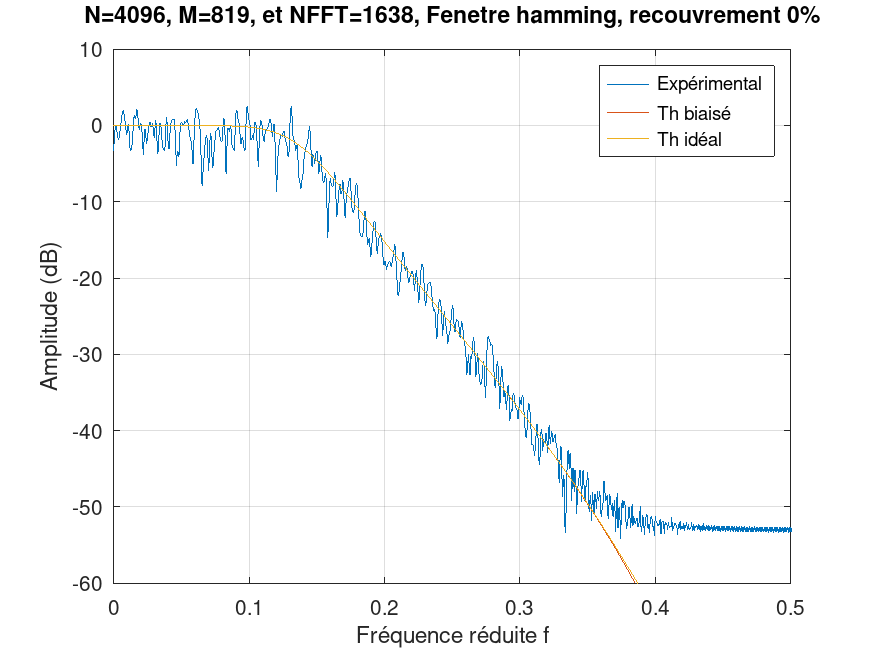
\includegraphics[width=\columnwidth]{Variation-recouvrement-0.png}
\caption{$N = 4096$ -- $M = 819$, $NFFT = 1638$. Choix de fenêtre = Hamming -- Recouvrement de $0\%$}
\end{figure}

\begin{figure}[H]
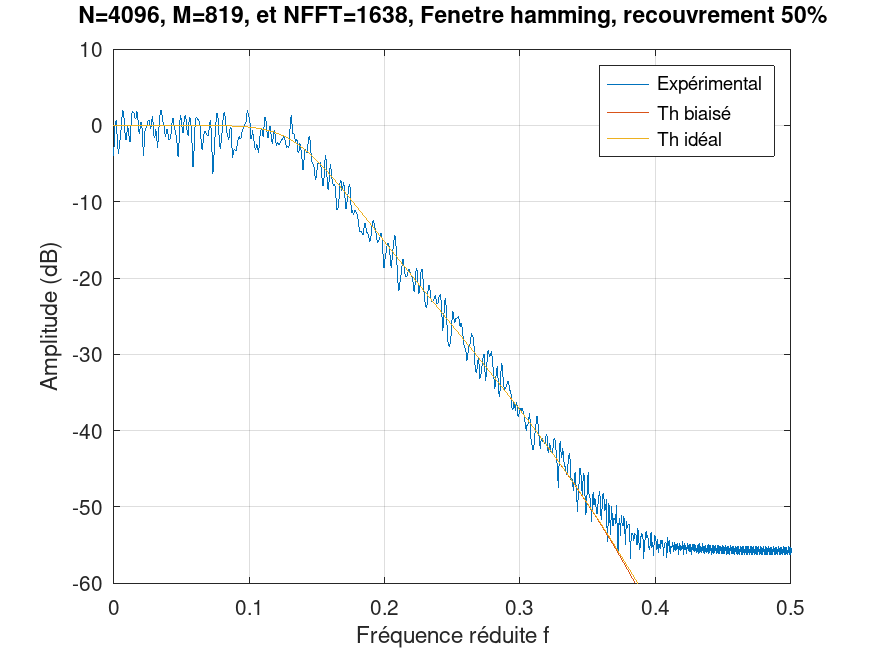
\includegraphics[width=\columnwidth]{Variation-recouvrement-0.5.png}
\caption{$N = 4096$ -- $M = 819$, $NFFT = 1638$. Choix de fenêtre = Hamming -- Recouvrement de $50\%$}
\end{figure}

\finrep

Que permet le recouvrement entre tranches ?

\debutrep{réponse ci-dessous}
Le recouvrement permet d'augmenter le nombre d'échantillons de chaque tranche (et donc la précision de la FFT), sans pour autant réduire le nombre de tranches.
Pour une fenetre de Hamming, on observe une légère réduction de la variance en bande passante ainsi qu'une légère diminution du biais en bande atténuée.

On observe cependant une grande amélioration de variance et biais par rapport à la fenêtre rectangulaire de l'estimateur moyenné.
\finrep

\item Etude du biais et de la variance en fonction de la fenêtre utilisée

Pour $N$, $M$ et $NFFT$ fixés et pour différents choix de fenêtre,  tracez les figures correspondantes aux conditions indiquées ci-dessous.

\debutrep{figure ci-dessous}
\begin{figure}[H]
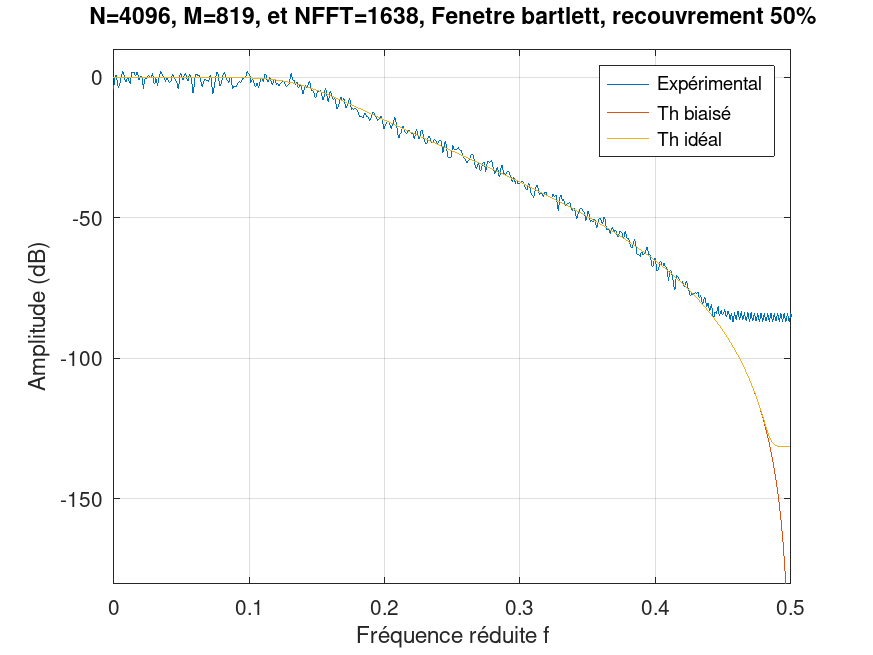
\includegraphics[width=\columnwidth]{Variation-fenetre-bartlett.png}
\caption{$N = 4096$ -- $M = 819$, $NFFT = 1638$. Fenêtre trianngle -- Recouvrement de $50\%$}
\end{figure}

\begin{figure}[H]
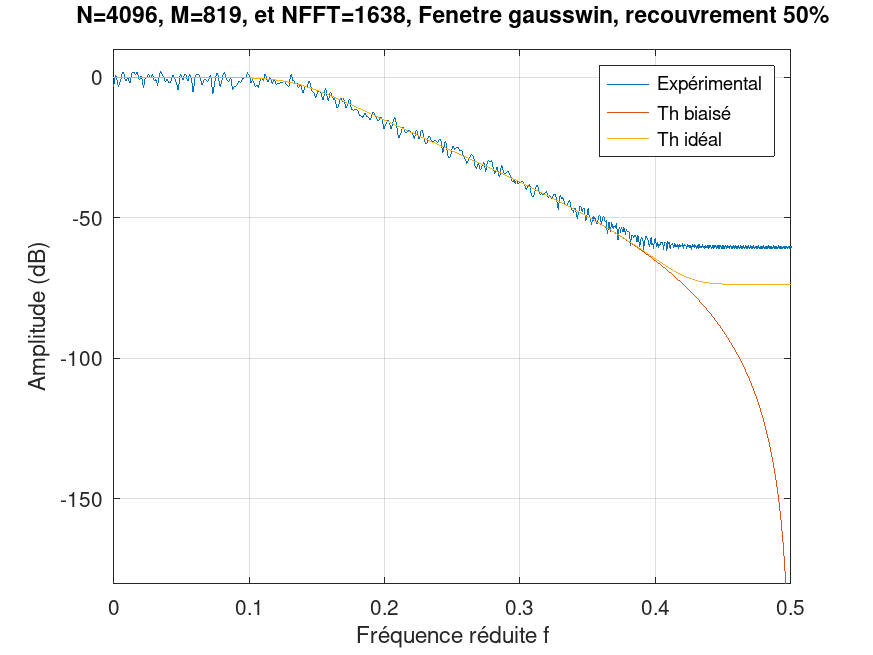
\includegraphics[width=\columnwidth]{Variation-fenetre-gausswin.png}
\caption{$N = 4096$ -- $M = 819$, $NFFT = 1638$. Fenêtre Gaussienne -- Recouvrement de $50\%$}
\end{figure}

\finrep

Que permet l'utilisation d'une fenêtre autre que rectangulaire ? Expliquer.

\debutrep{réponse ci-dessous}
Une fenêtre autre que rectanguaire permet d'éviter la convolution par un sinus cardinal dans le domaine spectral, augmentant alors la précision de l'estimation de la DSPM.

En observant la densité spectrale d'énergie, on peut aisément déduire que le spectre se rapprochant le plus d'un Dirac (élément neutre de la convolution) est l'estimateur dont la limitation temporelle affecte le moins la DSPM du signal.

On observe alors une amélioration descaractéristiques telles que la variance ou l'écart-type mais une diminution de la résolution fréquentielle, la fenêtre rectangulaire ayant le "pic" le plus fin sur sa DSPM.
\finrep

\end{enumerate}

Pour quelles valeurs des paramètres d'analyse obtenez vous le meilleur résultat (celui qui vous parait le plus satisfaisant)?

\debutrep{réponse ci-dessous}

Longueur de la séquence analysée $N = 20 000$ \\
Longueur des tranches $M = 0.2 * N = 4000 $ \\
Type de fenêtre Hanning \\
Taux de recouvrement =  50\%\\
Nombre de points de transformée de Fourier $NFFT = 2M = 8000$

\finrep

\section{Utilisation des estimateurs précédents pour analyser un signal inconnu}

\subsection{Modification des programmes}

Script d'une des fonctions modifiée

\debutrep{code ci-dessous}
\begin{verbatim}
close all;
clear variables;
clc;
%% Pour charger la bibliothèque signal
pkg load signal;

%% Charge le vecteur S
load sig

%% Première fonction
N = 100000;
NFFT = 2^17;
figure()
%appel de la fonction simple
[Gamma1,VecteurFreq1, N] = simpleDSPM(s,1,N, NFFT);
semilogy(VecteurFreq1,Gamma1)
axis([0 0.5 10 10^7])
figure()

%% Deuxième fonction
N = 100000;
M = 5000;
NFFT = 2^17;
[Gamma2, VecteurFreq2] = moyenneurDSPM(s, N, M, NFFT);
semilogy(VecteurFreq2,Gamma2)
axis([0 0.5 10 10^7])

%% Troisième fonction
N = 100000;
M = 5000;
NOVERLAP = 0.5;
NFFT = 2^17;
[Gamma3,VecteurFreq3] = welchDSPM(s,N,'hanning',M,NOVERLAP,NFFT);
figure()
semilogy(VecteurFreq3,Gamma3)
axis([0 0.5 10 10^7])

\end{verbatim}
\finrep
\newpage
\subsection{Expérimentation}

Afficher les spectres estimés obtenus avec chacune des 3 méthodes étudiées.

\debutrep{figure ci-dessous}
\begin{figure}[H]

\caption{Estimateur spectral simple. $N=100000, NFFT=2^{17}$.}
\end{figure}
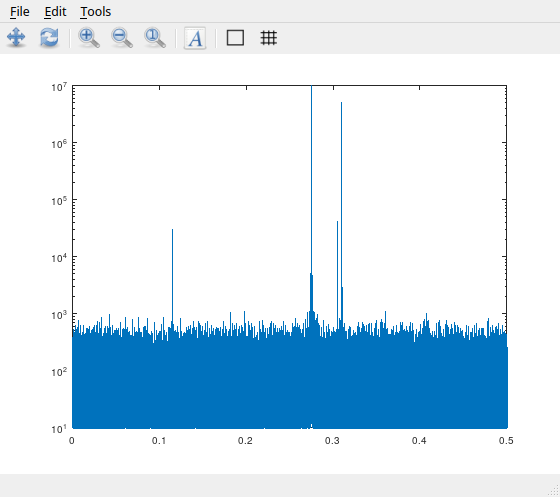
\includegraphics[width=\columnwidth]{Part4simple.png}
\begin{figure}[H]

\caption{Estimateur spectral moyenné. $N=100000, NFFT=2^{17}, M=5000$.}
\end{figure}
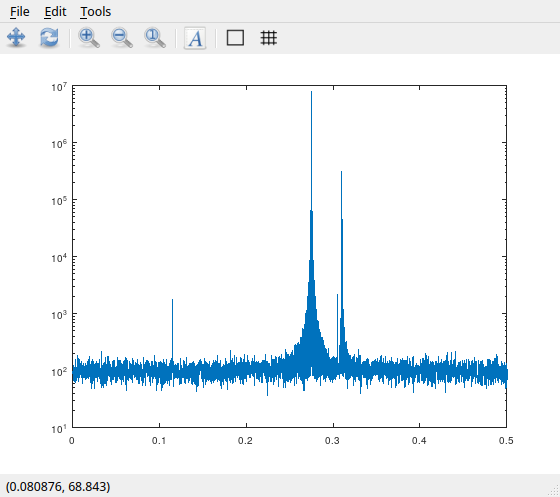
\includegraphics[width=\columnwidth]{Part4moy.png}
\begin{figure}[H]

\caption{Estimateur spectral de Welch. $N=100000, NFFT=2^{17}, M=5000$, fenetre de hanning, overlap de 0,5\%.}
\end{figure}
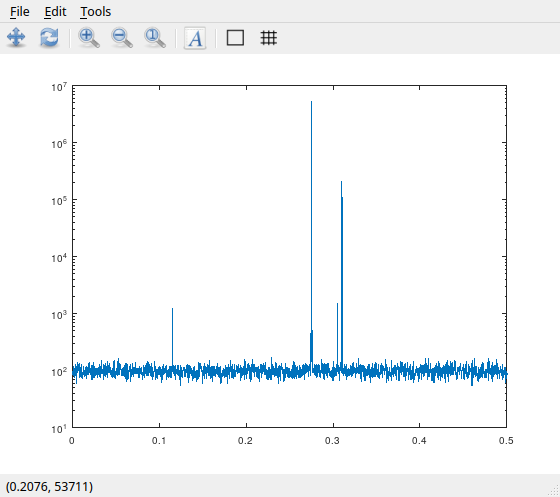
\includegraphics[width=\columnwidth]{Part4welc.png}
\finrep

Décrivez précisément la démarche expérimentale suivie. Avec quelle méthode êtes vous capable avec certitude de décrire le contenu fréquentiel de ce signal ?

\debutrep{réponse ci-dessous}
La méthode le plus adéquate pour faire l'étude du signal est celle de welsh, c'est celle qui est la moins bruitée
\finrep

\subsubsection{Interprétations}

\begin{enumerate}
\renewcommand{\theenumi}{\Alph{enumi}}

\item Que inconvénient majeur l'utilisation d'une fenêtre (d'apodisation en temps) engendre-t-elle?

\debutrep{réponse ci-dessous}
Elle diminue la résolution fréquentielle et engendre plus de calculs.
\finrep

\item Décrire (sans dessin) la forme de la DSPM obtenue.

\debutrep{réponse ci-dessous}
On a 0,275 pour le premier pic

0,31  pour le second pic

0,115 pour le troisième

0,305 pour quatrième
\finrep

\item Quelles informations la forme de cette DSPM apporte-t-elle sur le contenu (la nature) du signal?
\debutrep{réponse ci-dessous}
La DSPM permet d'avoir des information sur les fréquences du signal et sur la forme du bruit
\finrep

\item Quelles mesures concernant  les caractéristiques du signal peut-on effectuer sur la DSPM?

\debutrep{réponse ci-dessous}
On peut savoir où sont les fréquences du signal pour faire un filtrage adéquat
\finrep

\end{enumerate}

\end{document}








































